\documentclass{minimal}

\usepackage{tikz}
%\usetikzlibrary{trees,snakes}
\usepackage{verbatim}
\usepackage{pgf,tikz}
\usepackage{mathrsfs}
\usetikzlibrary{arrows}

%global definitions

\def\Rf{1cm}

\def\lpos{1.25331}
\def\lneg{-1.25331}

\def\lhalfpos{0.626655}
\def\lhalfneg{-0.626655}

\def\domlimpos{1.6}
\def\domlimneg{-1.6}

\def\loadlimpos{1.5}
\def\loadlimneg{-1.5}

\def\loadlabelpos{0.2}
\def\loadlabelneg{-0.2}

\def\thetabot{30}
\def\thetaup{60}
\def\thetavalue{45}
\def\thetaround{390}
\def\thetadraw{11.25}

\def\costhetabot{0.8660256}
\def\sinthetabot{0.5}

\def\costhetaup{0.5}
\def\sinthetaup{0.8660256}
  
\def\costheta{0.707107}
\def\sintheta{0.707107}

\def\xM{0.636396}
\def\yM{0.636396}
\def\xcrack{0.825253}
\def\ycrack{0.825253}

\def\drawparone{0.2}
\def\drawpartwo{0.3}
\def\drawparthree{0.6}
\def\drawparfour{-1.375}
\def\drawparfive{-0.433013}
\def\drawparsix{0.25}
\def\drawparseven{-0.05}
\def\drawpareight{0.75}
\def\drawparnine{0.852}
\def\drawparten{0.85}
\def\drawpareleven{0.52}
\def\drawpartwelve{0.259808}
\def\drawparthirteen{0.15}
\def\drawparfourteen{0.519615}
\def\drawparfifteen{0.212132}
\def\drawparsixteen{0.357009}
\def\drawparseventeen{0.273943}
\def\drawpareighteen{0.424264}
\def\drawparnineteen{-30.7096}
\def\drawpartwenty{120.71}
\def\drawpartwentyone{0.267084}
\def\drawpartwentytwo{0.60876142900872066}
\def\drawpartwentythree{0.79335334029123517}

\def\yarrowone{-1.12798}
\def\yarrowtwo{-1.00265}
\def\yarrowthree{-0.877317}
\def\yarrowfour{-0.751986}
\def\yarrowfive{-0.501324}
\def\yarrowsix{-0.375993}
\def\yarrowseven{-0.250662}
\def\yarroweight{-0.125331}
\def\yarrownine{0.}
\def\yarrowten{0.125331}
\def\yarroweleven{0.250662}
\def\yarrowtwelve{0.375993}
\def\yarrowthirteen{0.501324}
\def\yarrowfourteen{0.751986}
\def\yarrowfifteen{0.877317}
\def\yarrowsixteen{1.00265}
\def\yarrowseventeen{1.12798}

\begin{document}
\pagestyle{empty}

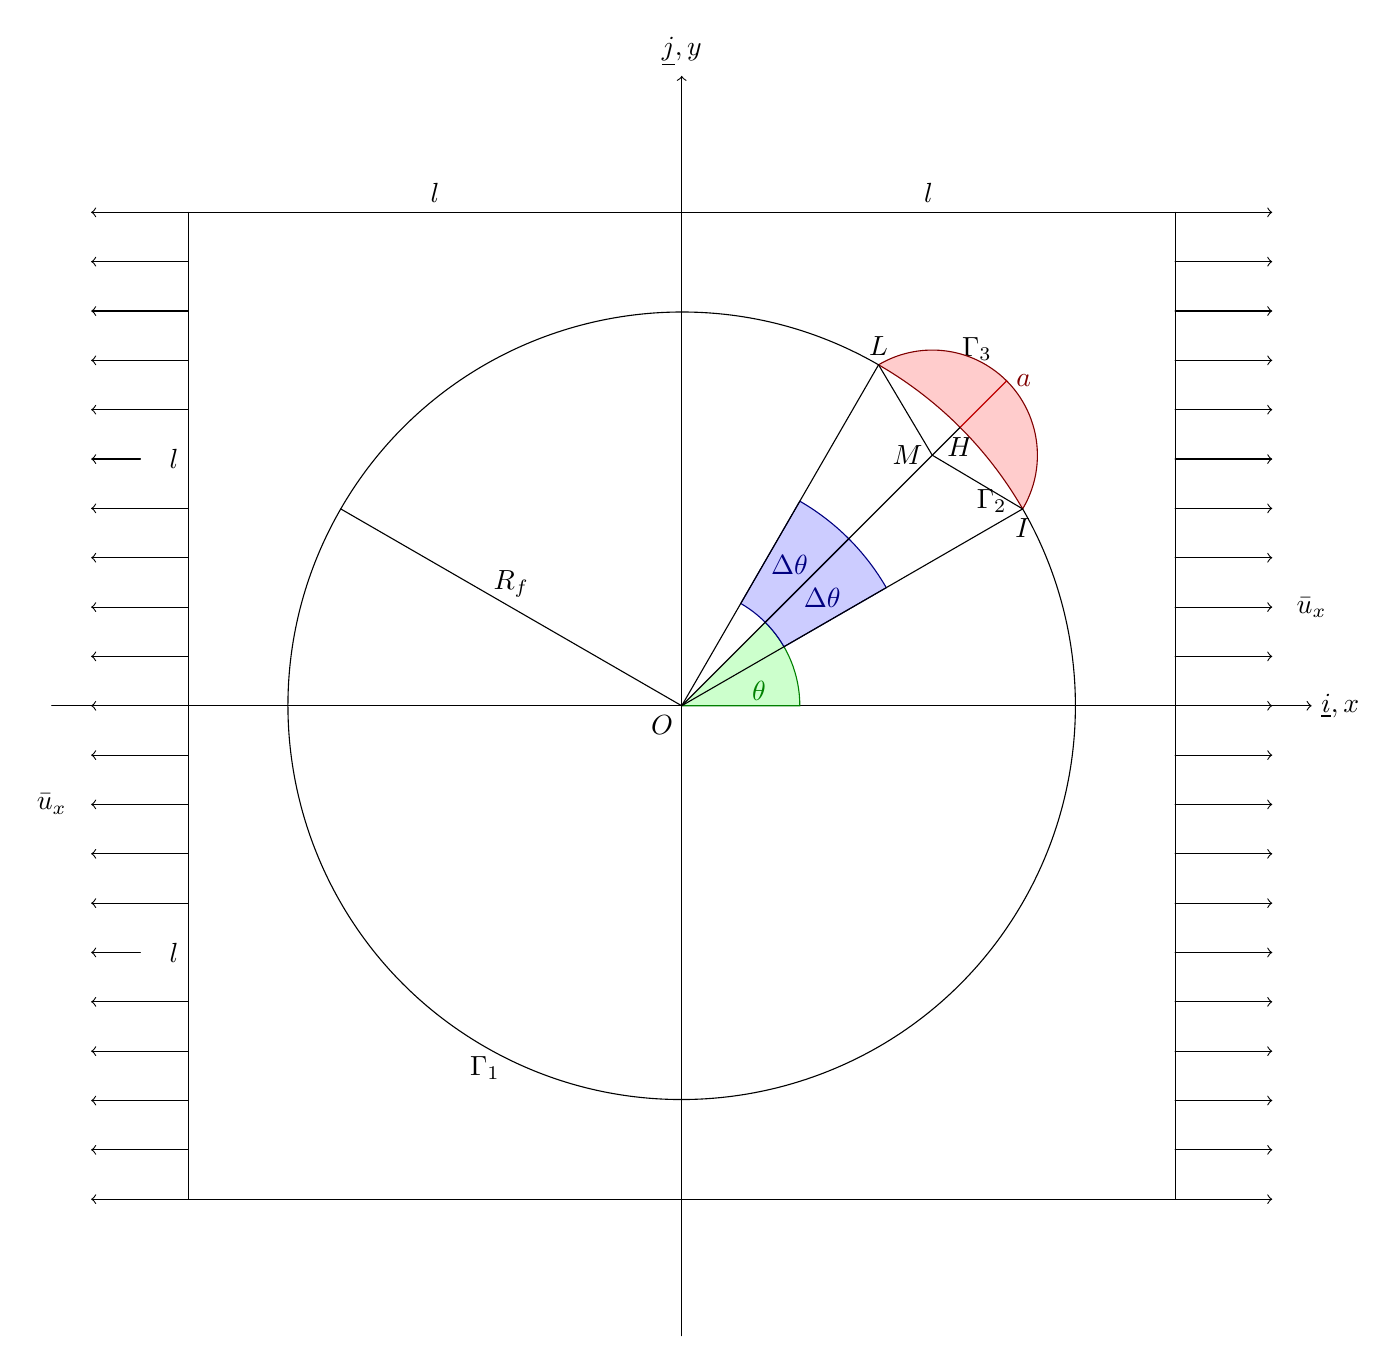
\begin{tikzpicture}[scale=5,cap=round]

\tikzstyle{axes}=[]

\draw (\costhetaup,\sinthetaup)arc (\thetaup:\thetaround:\Rf);

\begin{scope}[style=axes]
  \draw[->] (\domlimneg,0) -- (\domlimpos,0) node[right] {$\underline{i}, x$};
  \draw[->] (0,\domlimneg) -- (0,\domlimpos) node[above] {$\underline{j}, y$};
\end{scope}

\foreach \x in {\lneg, \yarrowone, \yarrowtwo, \yarrowthree, \yarrowfour, \lhalfneg, \yarrowfive, \yarrowsix, \yarrowseven, \yarroweight, \yarrownine, \yarrowten, \yarroweleven, \yarrowtwelve, \yarrowthirteen, \lhalfpos, \yarrowfourteen, \yarrowfifteen, \yarrowsixteen, \yarrowseventeen, \lpos}
 \draw[->] (\lpos,\x) -- (\loadlimpos,\x);

\foreach \x in {\lneg, \yarrowone, \yarrowtwo, \yarrowthree, \yarrowfour, \yarrowfive, \yarrowsix, \yarrowseven, \yarroweight, \yarrownine, \yarrowten, \yarroweleven, \yarrowtwelve, \yarrowthirteen,  \yarrowfourteen, \yarrowfifteen, \yarrowsixteen, \yarrowseventeen, \lpos}
\draw[->] (\lneg,\x) -- (\loadlimneg,\x);

\draw[->] (\drawparfour,\lhalfpos) -- (\loadlimneg,\lhalfpos);

\draw[->] (\drawparfour,\lhalfneg) -- (\loadlimneg,\lhalfneg);

\draw (\lneg,\lneg) -- (\lneg,\lpos);
\draw (\lneg,\lpos) -- (\lpos,\lpos) ;
\draw (\lpos,\lpos) -- (\lpos,\lneg);
\draw (\lpos,\lneg) -- (\lneg,\lneg);

\draw (\lneg,\lhalfpos) node[black,left] {$l$};
\draw (\lneg,\lhalfneg) node[black,left] {$l$};
\draw (\lhalfpos,\lpos) node[black,above] {$l$};
\draw (\lhalfneg,\lpos) node[black,above] {$l$};

\draw (\domlimpos,\loadlabelpos) node[black,above] {$\bar{u}_{x}$};
\draw (\domlimneg,\loadlabelneg) node[black,below] {$\bar{u}_{x}$};

\draw (\drawparfive,\drawparsix) node[black,above] {$R_{f}$};

\draw (\drawparseven,0) node[black,left,below] {$O$};

\draw (-\costhetaup,-\sinthetaup) node[black,below] {$\Gamma_{1}$};

\draw (\xM,\yM) node[black,left] {$M$};

\draw (\costhetabot,\sinthetabot) node[black,below] {$I$};

\draw (\costhetaup,\sinthetaup) node[black,above] {$L$};

\draw (\costheta,\sintheta) node[black,below] {$H$};

\draw (\xcrack,\ycrack) node[red!50!black,right] {$a$};

\draw (\drawpareight,\drawparnine) node[black,above] {$\Gamma_{3}$};

\draw (\drawparten,\drawpareleven) node[black,left] {$\Gamma_{2}$};

\filldraw[fill=green!20,draw=green!50!black] (0,0) -- (\drawpartwo,0pt) arc(0:\thetavalue:\drawpartwo);
\draw (\thetadraw:\drawparone) node[green!50!black] {$\theta$};

\filldraw[fill=blue!20,draw=blue!50!black](\drawpartwelve,\drawparthirteen) -- (\drawparfourteen,\drawpartwo) arc(\thetabot:\thetavalue:\drawparthree) --  (\drawparfifteen,\drawparfifteen) arc(\thetavalue:\thetabot:\drawpartwo);
\draw (\drawparsixteen,\drawparseventeen) node[blue!50!black] {$\Delta\theta$};

\filldraw[fill=blue!20,draw=blue!50!black](\drawparfifteen,\drawparfifteen) -- (\drawpareighteen,\drawpareighteen) arc(\thetavalue:\thetaup:\drawparthree) --  (\drawparthirteen,\drawpartwelve) arc(\thetaup:\thetavalue:\drawpartwo);
\draw (\drawparseventeen,\drawparsixteen) node[blue!50!black] {$\Delta\theta$};

\filldraw[fill=red!20,draw=red!50!black]([shift=(\drawparnineteen:\drawpartwentyone)]\xM,\yM) arc (\drawparnineteen:\drawpartwenty:\drawpartwentyone) --  (\costhetaup,\sinthetaup) arc(\thetaup:\thetabot:\Rf);


\draw[draw=red!75!black] (\costheta,\sintheta) -- (\xcrack,\ycrack);
\draw (0,0)--(\costheta,\sintheta);
\draw (0,0)--(\costhetabot,\sinthetabot);
\draw (0,0)--(-\costhetabot,\sinthetabot);
\draw (0,0)--(\costhetaup,\sinthetaup);
\draw (\xM,\yM)--(\costhetabot,\sinthetabot);
\draw (\xM,\yM)--(\costhetaup,\sinthetaup);

\end{tikzpicture}

\newpage

\begin{tikzpicture}[scale=5,cap=round]

\tikzstyle{axes}=[]

\draw (\costhetaup,\sinthetaup)arc (\thetaup:\thetaround:\Rf);

\begin{scope}[style=axes]
  \draw[->] (\domlimneg,0) -- (\domlimpos,0) node[right] {$\underline{i}, x$};
  \draw[->] (0,\domlimneg) -- (0,\domlimpos) node[above] {$\underline{j}, y$};
\end{scope}

\foreach \x in {\lneg, \yarrowone, \yarrowtwo, \yarrowthree, \yarrowfour, \lhalfneg, \yarrowfive, \yarrowsix, \yarrowseven, \yarroweight, \yarrownine, \yarrowten, \yarroweleven, \yarrowtwelve, \yarrowthirteen, \lhalfpos, \yarrowfourteen, \yarrowfifteen, \yarrowsixteen, \yarrowseventeen, \lpos}
 \draw[->] (\lpos,\x) -- (\loadlimpos,\x);

\foreach \x in {\lneg, \yarrowone, \yarrowtwo, \yarrowthree, \yarrowfour, \yarrowfive, \yarrowsix, \yarrowseven, \yarroweight, \yarrownine, \yarrowten, \yarroweleven, \yarrowtwelve, \yarrowthirteen,  \yarrowfourteen, \yarrowfifteen, \yarrowsixteen, \yarrowseventeen, \lpos}
\draw[->] (\lneg,\x) -- (\loadlimneg,\x);

\draw[->] (\drawparfour,\lhalfpos) -- (\loadlimneg,\lhalfpos);

\draw[->] (\drawparfour,\lhalfneg) -- (\loadlimneg,\lhalfneg);

\draw (\lneg,\lneg) -- (\lneg,\lpos);
\draw (\lneg,\lpos) -- (\lpos,\lpos) ;
\draw (\lpos,\lpos) -- (\lpos,\lneg);
\draw (\lpos,\lneg) -- (\lneg,\lneg);

\draw (\lneg,\lhalfpos) node[black,left] {$l$};
\draw (\lneg,\lhalfneg) node[black,left] {$l$};
\draw (\lhalfpos,\lpos) node[black,above] {$l$};
\draw (\lhalfneg,\lpos) node[black,above] {$l$};

\draw (\domlimpos,\loadlabelpos) node[black,above] {$\bar{u}_{x}$};
\draw (\domlimneg,\loadlabelneg) node[black,below] {$\bar{u}_{x}$};

\draw (\lpos,\lpos) node[black,above] {$\left(l,l\right)$}
\draw (\lneg,\lpos) node[black,above] {$\left(-l,l\right)$}

\draw (\lpos,\lneg) node[black,below] {$\left(l,-l\right)$}
\draw (\lneg,\lneg) node[black,below] {$\left(-l,-l\right)$}

\draw (0,\Rf) node[black,above] {$\left(0,R_{f}\right)$}
\draw (-\Rf,0) node[black,left] {$\left(-R_{f},0\right)$}
\draw (0,-\Rf) node[black,below] {$\left(0,-R_{f}\right)$}
\draw (\Rf,0) node[black,right] {$\left(R_{f},0\right)$}

\draw (\drawparfive,\drawparsix) node[black,above] {$R_{f}$};
\draw (\drawparseven,0) node[black,left,below] {$O$};
\draw (-\costhetaup,-\sinthetaup) node[black,below] {$\Gamma_{1}$};
\draw (\costhetabot,\sinthetabot) node[black,below] {$I$};
\draw (\costhetaup,\sinthetaup) node[black,above] {$L$};
\draw (\costheta,\sintheta) node[black,below] {$H$};
\draw (\costheta,\sintheta) node[red!50!black,above] {$a$};
\draw (\drawpartwentytwo,\drawpartwentythree) node[black,above] {$\Gamma_{3}$};
\draw (\drawparten,\drawpareleven) node[black,left] {$\Gamma_{2}$};

\filldraw[fill=green!20,draw=green!50!black] (0,0) -- (\drawpartwo,0pt) arc(0:\thetavalue:\drawpartwo);
\draw (\thetadraw:\drawparone) node[green!50!black] {$\theta$};

\filldraw[fill=blue!20,draw=blue!50!black](\drawpartwelve,\drawparthirteen) -- (\drawparfourteen,\drawpartwo) arc(\thetabot:\thetavalue:\drawparthree) --  (\drawparfifteen,\drawparfifteen) arc(\thetavalue:\thetabot:\drawpartwo);
\draw (\drawparsixteen,\drawparseventeen) node[blue!50!black] {$\Delta\theta$};

\filldraw[fill=blue!20,draw=blue!50!black](\drawparfifteen,\drawparfifteen) -- (\drawpareighteen,\drawpareighteen) arc(\thetavalue:\thetaup:\drawparthree) --  (\drawparthirteen,\drawpartwelve) arc(\thetaup:\thetavalue:\drawpartwo);
\draw (\drawparseventeen,\drawparsixteen) node[blue!50!black] {$\Delta\theta$};

\draw[draw=red](\costhetaup,\sinthetaup) arc(\thetaup:\thetabot:\Rf);


\draw (0,0)--(\costheta,\sintheta);
\draw (0,0)--(\costhetabot,\sinthetabot);
\draw (0,0)--(-\costhetabot,\sinthetabot);
\draw (0,0)--(\costhetaup,\sinthetaup);


\end{tikzpicture}

\end{document}